В данной главе рассматривается задача выбора структуры модели глубокого обучения. Предлагается ввести вероятностные предположения о распределениях параметров и структуры модели. 
Проводится градиентная оптимизация параметров и гиперпараметров модели на основе байесовского вариационного вывода.  В качестве оптимизируемой функции для гиперпараметров модели предлагается обобщенная функция обоснованности. Показано, что данная функция позволяет проводить оптимизацию, соответствующую нескольким критериям выбора структуры модели: методу максимального правдоподобия, последовательному увеличению и снижению сложности модели, полному перебору структуры модели, а также получению максимума вариационной оценки обоснованности модели. Решается двухуровневая задача оптимизации: на первом уровне проводится оптимизация нижней оценки обоснованности модели по вариационным параметрам модели. На втором уровне проводится оптимизация гиперпараметров модели.

\section{Вероятностная модель}
Определим априорные распределения параметров и структуры модели следующим образом.
Пусть параметры модели распределены нормально с нулевым средним:
\[
    \mathbf{w}^{i,j}_k \sim \mathcal{N}\bigl(\mathbf{0}, \gamma^{i,j}_k(\mathbf{A}^{i,j}_k)^{-1}\bigr),
\]
где $ (\mathbf{A}^{i,j}_k)^{-1}$ --- диагональная матрица. Апирорное распределение $p(\mathbf{w}|\boldsymbol{\Gamma}, \mathbf{h})$ параметров $\mathbf{w}^{i,j}_k$ зависит не только от гиперпараметров $\mathbf{A}_k^{i,j}$, но и от структурного параметра $\gamma^{i,j}_k$.


В качестве априорного распределения для структуры $\boldsymbol{\Gamma}$ предлагается использовать произведение распределений Gumbel-Softmax~\cite{gs}:
\[
    p(\boldsymbol{\Gamma}|\mathbf{h},\boldsymbol{\lambda}) = \prod_{(j,k) \in E} p(\boldsymbol{\gamma}^{j,k}|\mathbf{s}, \lambda_\text{temp}),
\]
где для каждого структурного параметра $\boldsymbol{\gamma}$ с количеством базовых функций $K$ вероятность $p(\boldsymbol{\gamma}|\mathbf{s}, \lambda_\text{temp})$ определна следующим образом:
\[
    p(\boldsymbol{\gamma}|\mathbf{s}, \lambda_\text{temp}) = (K-1)!\lambda_{\text{temp}}^{K-1}\prod_{l=1}^K s_l\gamma_l^{-\lambda_\text{temp} -1} \left(\sum_{l=1}^K s_l\gamma_l^{-\lambda_\text{temp}}\right)^{-K},
\]
где $\mathbf{s} \in (0,\infty)^K$ --- гиперпараметр, отвечающий за смещенность плотности распределения относительно точек симплекса на $K$ вершинах, $\lambda_{\text{temp}}$ --- метапараметр температуры, отвечающий за концентрацию плотности вблизи вершин симплекса или в центре симплекса.

Перечислим свойства, которыми обладает распределение Gumbel-Softmax:
\begin{enumerate}
\item Реализацию $\hat{\gamma}_l,$ т.е. $l$-й компоненты случайной величины $\boldsymbol{\gamma}$  можно породить следующим образом:
\[
    \hat{\gamma}_l = \frac{\text{exp}(\text{log}s_l+\hat{g}_l)/\lambda_{\text{temp}}}{\sum_{l'=1}^{K}\text{exp}(\text{log}s_{l'}+\hat{g}_{l'})/\lambda_{\text{temp}}},
\]
где $\hat{\mathbf{g}} \sim -\text{log}\bigl(-\text{log}~\mathcal{U}(0,1)^K\bigr).$ 

\item Свойство округления: $p(\gamma_{l_1} > \gamma_{l_2}, l_1\neq l_2|\mathbf{s}, {\lambda}_\text{temp}) = \frac{s_l}{\sum_{l'}s_{l'}}.$

\item При устремлении температуры к нулю реализация случайной величины концентрируется на вершинах симплекса:
\[
    p(\lim_{\lambda_{\text{temp}} \to 0}  \gamma_{l} = 1|\mathbf{s}, {\lambda}_\text{temp})  = \frac{s_l}{\sum_{l'}s_{l'}}.
\]


\item При устремлении температуры к бесконечности плотность распределения концентрируется в центре симплекса:
\begin{equation}
\label{eq:theorem_gs}
    \lim_{\lambda_{\text{temp}} \to \infty}  p(\boldsymbol{\gamma}|\mathbf{s}, {\lambda}_\text{temp}) = 
    \begin{cases}
    \infty, \boldsymbol{\gamma}_l = \frac{1}{K}, l \in \{1,\dots,K\},\\
    0, \text{ иначе.}
    \end{cases}
\end{equation}
\end{enumerate}

Доказательства первых трех утверждений приведены в~\cite{gumbel}. Докажем утверждение 4.

\begin{proof} 
Формула плотности записывается следующим образом с точностью до множителя:
\[
       \frac{\lambda_{\text{temp}}^{K-1}}{\left(\sum_{l=1}^K s_l\gamma_l^{-\frac{-K-1}{K}\lambda_\text{temp}}\sum_{l'=1}^K [l \neq l']s_l\gamma_l^{-\frac{1}{K}\lambda_\text{temp}}\right)^{K}}
\]


Заметим, что числитель $\lambda_{\text{temp}}^{K-1}$ имеет меньшую скорость сходимости, чем знаменатель. 
Знаменатель является суммой слагаемых вида:
\begin{equation}
\label{eq:gs}
    \left(\frac{\prod_{l' \neq l} \gamma_{l'}^{\frac{1}{K}}}{\gamma_l^{\frac{K-1}{K}}}\right)^{\lambda_{\text{temp}}}.
\end{equation}
Пусть хотя бы для одного $l$: $\gamma_l \neq \frac{1}{K}$. Пусть $l'$ соответствует индексу максимальной компоненты вектора $\boldsymbol{\gamma}$.
Для $l=l'$ предел выражения~\eqref{eq:gs} при $\lambda_{\text{temp}}$ стремится к бесконечности. Для $l\neq l'$ предел выражения~\eqref{eq:gs} при $\lambda_{\text{temp}}$ стремится к нулю. Возводя сумму пределов в степень $-K$ получаем предел плотности, равный нулю.

Пусть $\boldsymbol{\gamma} = \frac{1}{K}$.
Тогда выражение с точностью до множителя упрощается до $\lambda^{K-1}$. Предел данного выражения стремится к бесконечности.
Таким образом, предел плотности Gumbel-Softmax равен выражению~\eqref{eq:theorem_gs}, что и требовалось доказать.

\end{proof}


Первое свойство Gumbel-Softmax распределения позволяет использовать репараметризацию при вычислении градиента в вариационном выводе (англ. reparametrization trick). 
Идея подхода заключается в следующем. Рассмотрим для примера математическое ожидание логарифма правдоподобия выборки модели по некоторому непрерывному распределению $q$:
\[
    \mathsf{E}_q \text{log}~p(\mathbf{y}|\mathbf{w}, \mathbf{X}, \mathbf{h}, \boldsymbol{\lambda})=  \int_{\mathbf{w}} \text{log}~p(\mathbf{y}|\mathbf{w}, \mathbf{X}, \mathbf{h}, \boldsymbol{\lambda})q(\mathbf{w})d\mathbf{w}.
\]
Продиффиринцируем данное выражение по параметрам $\boldsymbol{\theta}$ вариационного распределения $q$:
\[
    \nabla_{\boldsymbol{\theta}} \mathsf{E}_q \text{log}~p(\mathbf{y}|\mathbf{w}, \mathbf{X}, \mathbf{h}, \boldsymbol{\lambda}) = \int_{\mathbf{w}}  \nabla_{\boldsymbol{\theta}}\text{log}~p(\mathbf{y}|\mathbf{w}, \mathbf{X}, \mathbf{h}, \boldsymbol{\lambda})q(\mathbf{w})d\mathbf{w} + \int_{\mathbf{w}}  \text{log}~p(\mathbf{y}|\mathbf{w}, \mathbf{X}, \mathbf{h}, \boldsymbol{\lambda})\nabla_{\boldsymbol{\theta}}q(\mathbf{w})d\mathbf{w}.
\]
Первое слагаемое в общем видел сложновычислимо. Пусть распределение $q$ можно представить как функцию от непараметрического распределения:
\[
    q(\mathbf{w}) = q(g(\varepsilon)).
\]
Тогда 
\[
 \nabla_{\boldsymbol{\theta}} \mathsf{E}_q \text{log}~p(\mathbf{y}|\mathbf{w}, \mathbf{X}, \mathbf{h}, \boldsymbol{\lambda}) = \nabla_{\boldsymbol{\theta}} \mathsf{E}_{\varepsilon} \text{log}~p(\mathbf{y}|\mathbf{w}, \mathbf{X}, \mathbf{h}, \boldsymbol{\lambda}) = \int_{\varepsilon}  \nabla_{\boldsymbol{\theta}} \text{log}~p(\mathbf{y}|\mathbf{w}, \mathbf{X}, \mathbf{h}, \boldsymbol{\lambda})  p(\varepsilon) d\varepsilon.
\]
Таким образом, распределение, позволяющее произвести репараметризацию, является более удобным для вычисления интегральных оценок.
Кроме того, данный подход позволяет значительно повысить точность вычисления градиента от функций, зависящих от случайных величин~\cite{reparametrization}.
% отсюда: http://gregorygundersen.com/blog/2018/04/29/reparameterization/

Пример распределения Gumbel-Softmax при различных параметрах представлен на Рис.~\ref{fig:gs}. В качестве альтернативы для априорного распределения на структуре выступает  распределение Дирихле и равномерное распределение. Выбор в качестве распределения на структуре произведения Gumbel-Softmax распределения обоснован выбором этого же распределения в качестве вариационного. 

\begin{figure}
 \begin{minipage}[t]{.2\textwidth}
        \centering
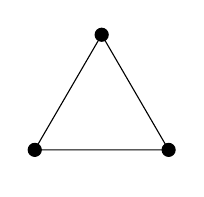
\begin{tikzpicture}[%
x={(1.7cm,0cm)},
y={(0cm,1.7cm)},
]

\coordinate (A) at (0,0); 
\coordinate (B) at (1,0) ;
\coordinate (C) at (0.5,0.86); 

%Ecken
\node[circle,scale=0.5,fill=black,draw=black](Ap) at (0,0){};
\node[circle,scale=0.5,fill=black,draw=black](Bp) at (1,0){};
\node[circle,scale=0.5,fill=black,draw=black](Cp) at (0.5,0.86){};

%Kanten
\draw[] (A)
-- (B)  node[midway, below]{}
-- (C)      node[midway, right]{}
-- (A)  node[midway, left]{};

\end{tikzpicture}
\subcaption{}
\end{minipage}
\hfill
 \begin{minipage}[t]{.2\textwidth}
   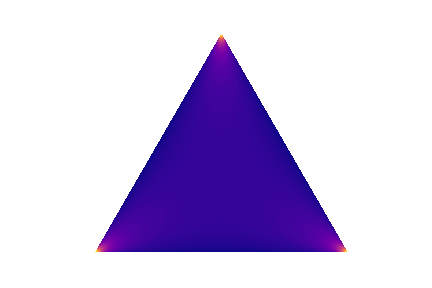
\includegraphics[width=\textwidth]{plots/notebooks/gs1.png}
\subcaption{}
\end{minipage}
\hfill
 \begin{minipage}[t]{.2\textwidth}
   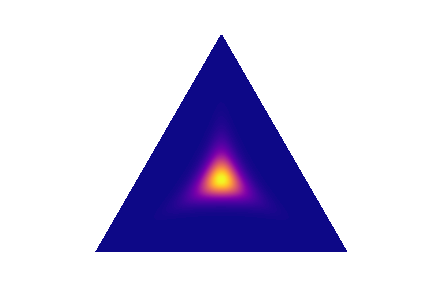
\includegraphics[width=\textwidth]{plots/notebooks/gs5.png}
\subcaption{}
\end{minipage}
\hfill
 \begin{minipage}[t]{.2\textwidth}
   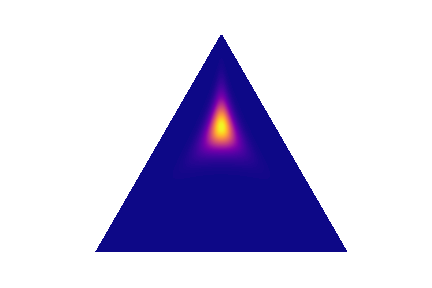
\includegraphics[width=\textwidth]{plots/notebooks/gs5_shift.png}
\subcaption{}
\end{minipage}

\caption{Пример распределения Gumbel-Softmax при различных значениях параметров: а)~$\lambda_{temp}\to0$, б)~$\lambda_{temp}=1, \mathbf{s}=[1,1,1]$, в)~$\lambda_{temp}=5, \mathbf{s}=[1,1,1]$, г)~$\lambda_{temp}=5, \mathbf{s}=[10,0.1,0.1].$}
\label{fig:gs}

\end{figure}


Заметим, что предлагаемое априорное распределение неоднозначно: одно и то же распределение  можно получить с различными значениями гиперпарамета $\mathbf{A}^{i,j}_k$ и структурного параметра $\gamma^{i,j}_k$. В качестве регуляризатора для матрицы $(\mathbf{A}^{i,j}_k)^{-1}$ предлагается использовать обратное гамма-распределение:
\[
    (\mathbf{A}^{i,j}_k)^{-1} \sim \text{inv-gamma}(\lambda_1,\lambda_2),
\]
где $\lambda_1,\lambda_2 \in \boldsymbol{\lambda}$ --- метапараметры оптимизации. 
Использование обратного гамма-распределения в качестве распределения гиперпараметров можно найти в~\cite{bishop,mackay}. В данной работе обратное распределение выступает как регуляризатор гиперпараметров.
Калибруя метапарамы   $\lambda_1,\lambda_2$ можно получить более сильную или более слабую регуляризацию~\cite{rvm}. Пример распределений $\text{inv-gamma}(\lambda_1,\lambda_2)$ для разных значений метапараметров $\lambda_1,\lambda_2$ изображен на Рис.~\ref{fig:inv-gamma}.

\begin{figure}
\centering
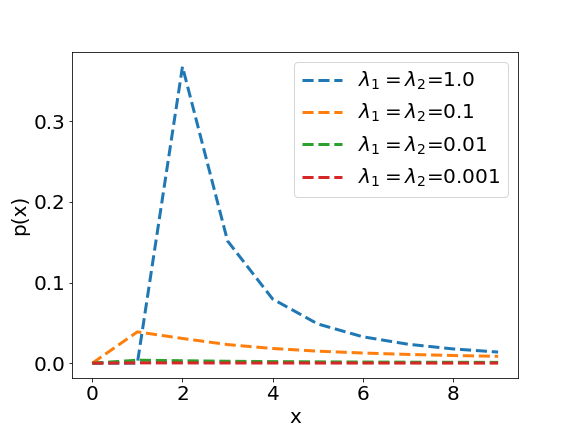
\includegraphics[width=0.6\textwidth]{plots/notebooks/invgamma.png}
\caption{Графики обратных гамма распределений для различных значений метапараметров.}
\label{fig:inv-gamma}
\end{figure}


Таким образом, предлагаемая вероятностная модель содержит следующие компоненты:
\begin{enumerate}
\item Параметры $\mathbf{w}$ модели, распределенные нормально.
\item Структура модели $\boldsymbol{\Gamma}$ распределены по распределению Gumbel-Softmax.
\item Гиперпараметры: $\mathbf{h} = [\text{diag}(\mathbf{A}), \mathbf{s}]$, где $\mathbf{A}$ --- конкатенация матриц $\mathbf{A}^{j,k}, (j,k) \in E,$ $\mathbf{s}$ --- конкатенация параметров Gumbel-Softmax распределений $\mathbf{s}^{j,k}, (j,k) \in E$, где $E$ --- множество ребер, соответствующих графу рассматриваемого параметрического семейства.
\item Метапараметры: $\boldsymbol{\lambda} = [\lambda_1, \lambda_2].$
\end{enumerate}

График вероятностной модели в формате плоских нотаций представлен на Рис.~\ref{fig:plate_prob}.
\begin{figure}
\centering
   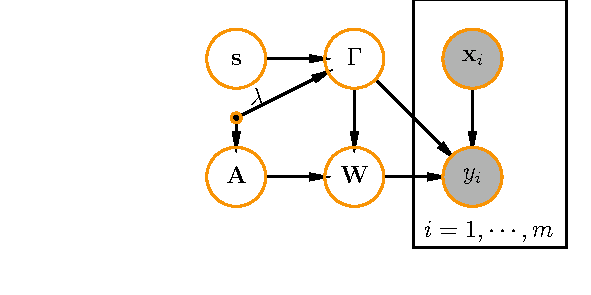
\includegraphics[width=0.5\textwidth]{plots/notebooks/simple_plate.pdf}
\caption{График предлагаемой вероятностной модели в формате плоских нотаций. Переменные обозначены белыми и серыми кругами, константы обозначены обведенными черными кругами. Наблюдаемые переменные обозначены серыми кругами.}
\label{fig:plate_prob}
\end{figure}

\section{Вариационная оценка для обоснованности вероятностной модели}
В качестве критерия выбора структуры модели предлагается использовать апостериорную вероятность гиперпараметров:
\begin{equation}
\label{eq:optimal_hyper}
    p(\mathbf{h}|\mathbf{y}, \mathbf{X}, \boldsymbol{\lambda}) \propto p(\mathbf{y}|\mathbf{X}, \mathbf{h}, \boldsymbol{\lambda}) p(\mathbf{h}|\boldsymbol{\lambda}) \to \max_{\mathbf{h} \in \mathbb{H}},
\end{equation}
где структура модели и параметры модели выбираются на основе полученных значений гиперпараметров:
\[
    \boldsymbol{\Gamma}^* = \argmax_{\boldsymbol{\Gamma} \in \amsmathbb{\Gamma}} p(\boldsymbol{\Gamma}|\mathbf{y}, \mathbf{X}, \mathbf{h}^*),
\]
\[
    \mathbf{w}^* = \argmax_{\mathbf{w} \in \mathbb{W}} p(\mathbf{w}|\mathbf{y}, \mathbf{X}, \boldsymbol{\Gamma}^*, \mathbf{h}^*),
\]
где $\mathbf{h}^*$ --- решение задачи оптимизации~\eqref{eq:optimal_hyper}.

Для вычисления обоснованности $$p(\mathbf{y}|\mathbf{X}, \mathbf{h}, \boldsymbol{\lambda}) = \iint_{\boldsymbol{\Gamma},\mathbf{w}}p(\mathbf{y}|\mathbf{X}, \mathbf{w}, \boldsymbol{\Gamma},\boldsymbol{\lambda})p(\mathbf{w}|\boldsymbol{\Gamma},\mathbf{h}, \boldsymbol{\lambda})p(\boldsymbol{\Gamma}|\mathbf{h}, \boldsymbol{\lambda})d\boldsymbol{\Gamma}d\mathbf{w}$$ из~\eqref{eq:optimal_hyper} предлагается использовать вариационную оценку обоснованности.

\begin{theorem}
Пусть $q(\mathbf{w},\boldsymbol{\Gamma}|\boldsymbol{\theta})  = q(\mathbf{w},\boldsymbol{\Gamma}|\boldsymbol{\theta}_\mathbf{w})q_{\boldsymbol{\Gamma}}(\boldsymbol{\Gamma}|\boldsymbol{\theta}_{\boldsymbol{\Gamma}})$ --- вариационное распределение c параметрами $\boldsymbol{\theta}= [\boldsymbol{\theta}_\mathbf{w},\boldsymbol{\theta}_{\boldsymbol{\Gamma}} ]$, аппроксимирующее апостериорное распределение структуры и параметров:
\[
    q(\mathbf{w},\boldsymbol{\Gamma}|\boldsymbol{\theta}) \approx p(\mathbf{w},\boldsymbol{\Gamma}|\mathbf{y}, \mathbf{X}, \mathbf{h}, \boldsymbol{\lambda}),
\]
\[
    q_{\mathbf{w}}(\mathbf{w}|\boldsymbol{\theta}_\mathbf{w},\boldsymbol{\Gamma}) \approx p(\mathbf{w}|\mathbf{y}, \mathbf{X},  \boldsymbol{\Gamma},\mathbf{h}, \boldsymbol{\lambda}),
\]
\[
    q_{\boldsymbol{\Gamma}}(\boldsymbol{\Gamma}|\boldsymbol{\theta}_{\boldsymbol{\Gamma}}) \approx p(\boldsymbol{\Gamma}|\mathbf{y}, \mathbf{X},  \mathbf{h}, \boldsymbol{\lambda}).
\]

Тогда справедлива следующая оценка:
\begin{equation}
\label{eq:full_elbo}
\text{log} p(\mathbf{y}|\mathbf{X}, \mathbf{h}, \boldsymbol{\lambda}) \geq
\end{equation}
\[
 \mathsf{E}_{\boldsymbol{\Gamma} \sim q_{\boldsymbol{\Gamma}}}\mathsf{E}_{\mathbf{w} \sim q_{\mathbf{w}}} \text{log}p(\mathbf{y}|\mathbf{w}, \boldsymbol{\Gamma}, \mathbf{X}) - D_\text{KL}\left(q_{\boldsymbol{\Gamma}}(\boldsymbol{\Gamma}|\boldsymbol{\theta}_{\boldsymbol{\Gamma}})|p(\boldsymbol{\Gamma}|\mathbf{h}, \boldsymbol{\lambda})\right) - D_\text{KL}\left(q_{\mathbf{w}}(\mathbf{w}|\boldsymbol{\theta}_\mathbf{w},\boldsymbol{\Gamma})|p(\mathbf{w}|\boldsymbol{\Gamma}, \mathbf{h})\right),
\]
где $D_\text{KL}\left(q_{\mathbf{w}}(\mathbf{w}|\boldsymbol{\theta}_\mathbf{w},\boldsymbol{\Gamma})|p(\mathbf{w}|\boldsymbol{\Gamma}, \mathbf{h})\right)$ вычисляется по формуле условной дивергенции~\cite{TODO}:
\[
D_\text{KL}\left(q_{\mathbf{w}}(\mathbf{w}|\boldsymbol{\theta}_\mathbf{w},\boldsymbol{\Gamma})|p(\mathbf{w}|\boldsymbol{\Gamma}, \mathbf{h})\right) = \mathsf{E}_{\boldsymbol{\Gamma} \sim q_{\boldsymbol{\Gamma}}} \mathsf{E}_{\mathbf{w} \sim q_{\mathbf{w}}} \frac{\text{log}q(\mathbf{w}|\boldsymbol{\Gamma})}{\text{log}p(\mathbf{w}|\mathbf{h},\boldsymbol{\Gamma})}.
\]
\end{theorem}

\begin{proof}
Используя неравенство Йенсена получим 
\[
\text{log} p(\mathbf{y}|\mathbf{X}, \mathbf{h}, \boldsymbol{\lambda}) \geq
\]
\[
   \mathsf{E}_{q} \text{log}p(\mathbf{y}|\mathbf{w}, \boldsymbol{\Gamma}, \mathbf{X}) - D_\text{KL}(q (\mathbf{w},\boldsymbol{\Gamma}|\boldsymbol{\theta})|p(\mathbf{w},\boldsymbol{\Gamma}|\mathbf{h})).
\]

Декомпозируем распределение $q$ по свойству условной дивергенции:
\[
D_\text{KL}(q (\mathbf{w},\boldsymbol{\Gamma}|\boldsymbol{\theta})|p(\mathbf{w},\boldsymbol{\Gamma}|\mathbf{h})) = D_\text{KL}\left(q_{\boldsymbol{\Gamma}}(\boldsymbol{\Gamma}|\boldsymbol{\theta}_{\boldsymbol{\Gamma}})|p(\boldsymbol{\Gamma}|\mathbf{h}, \boldsymbol{\lambda})\right) + D_\text{KL}\left(q_{\mathbf{w}}(\mathbf{w}|\boldsymbol{\theta}_\mathbf{w},\boldsymbol{\Gamma})|p(\mathbf{w}|\boldsymbol{\Gamma}, \mathbf{h})\right).    
\]
\end{proof}

В качестве вариационного распределения $q_{\mathbf{w}}$ предлагается использовать нормальное распределение, не зависящее от структуры модели $\boldsymbol{\Gamma}$:
\[
    q_{\mathbf{w}} = \mathcal{N}(\boldsymbol{\mu}, \mathbf{A}_q), 
\]
где $\mathbf{A}_q$ --- диагональная матрица с диагональю $\boldsymbol{\alpha}_q$.

В качестве вариационного распределения $q_{\boldsymbol{\Gamma}}$ предлагается использовать произведение распределений Gumbel-Softmax. Конкатенацию параметров концентрации распределений обозначим $\mathbf{s}_q$. Его температуру обозначим $\theta_\text{temp}$.

Вариационными параметрами распределения $q$ являются параметры распределений $q_{\mathbf{w}}, q_{\boldsymbol{\Gamma}}$:
\[
    \boldsymbol{\theta} = [\boldsymbol{\mu}, \boldsymbol{\alpha}_q, \mathbf{s}_q, \theta_\text{temp}]. 
\]


График вероятностной вариационной модели в формате плоских нотаций представлен на Рис.~\ref{fig:plate_qprob}.
\begin{figure}
\centering
   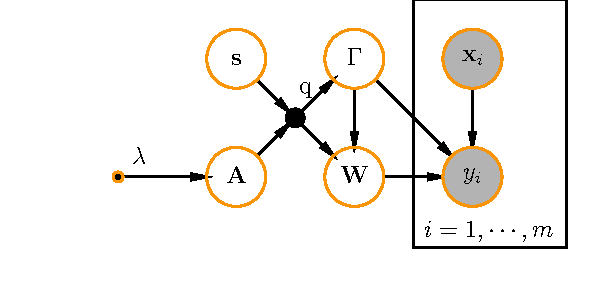
\includegraphics[width=0.5\textwidth]{plots/notebooks/plate.pdf}
\caption{График предлагаемой вероятностной вариационной модели в формате плоских нотаций. Переменные обозначены белыми и серыми кругами, константы обозначены обведенными черными кругами. Вариационное распределение обозначено черным кругом. Наблюдаемые переменные обозначены серыми кругами.}
\label{fig:plate_qprob}
\end{figure}

Для анализа сложности полученной модели введем понятие \textit{параметрической сложности}. 
\begin{defin} 
Параметрической сложностью  $C_p(\boldsymbol{\theta})$ модели с вариационными параметрами $\boldsymbol{\theta}$ на компакте $U_\mathbf{h} \subset \mathbb{H}$ назовем минимальную дивергенцию между вариационным и априорным распределением:
\[
C_p(\boldsymbol{\theta}|U_\mathbf{h}) = \min_{\mathbf{h} \in U_\mathbf{h}} \text{D}_\text{KL}\left(q(\mathbf{w}, \boldsymbol{\Gamma}|\boldsymbol{\theta})|p(\mathbf{w}, \boldsymbol{\Gamma}|\mathbf{h})\right).
\]
\end{defin}
Параметрическая сложность модели соответствует ожидаемой длине описания параметров модели при условии заданного параметрического априорного распределения~\cite{hinton_mdl}.

Одним из критериев удаления неинформативных параметров в вероятностных моделях является отношение вариационной плотности параметров в моде распределения к вариационной плотности параметра в нуле~\cite{nips}:
\[
    \frac{q_\mathbf{w}(\mu|\boldsymbol{\theta}_\mathbf{w})}{q(0|\boldsymbol{\theta}_\mathbf{w})} = \text{exp}\left(-\frac{2\alpha_q^2}{\mu^2}\right),
\]
где $q_\mathbf{w}(w|\boldsymbol{\theta}_\mathbf{w}) \sim \mathcal{N}(\mu, \alpha_q).$

Обобщим понятие относительной вариационной плотности на случай произвольных распределений.
\begin{defin}
Относительной вариационной   плотностью параметра $w \in \mathbf{w}$  при условии структуры $\boldsymbol{\Gamma}$ и гиперпараметров $\mathbf{h}$ назовем отношение моды вариационного распределения параметра к моде априорного распределению параметра:
\[
    \rho(w|\boldsymbol{\Gamma}, \boldsymbol{\theta}_\mathbf{w}, \mathbf{h},\boldsymbol{\lambda}) = \frac{q\bigl(\text{mode}~q\left(w|\boldsymbol{\Gamma}, \boldsymbol{\theta}_\mathbf{w}\right)|\boldsymbol{\Gamma}, \boldsymbol{\theta}_\mathbf{w}\bigr)}{q\bigl(\text{mode}~p\left({w}|\boldsymbol{\Gamma}, \mathbf{h},\boldsymbol{\lambda}\right)|\boldsymbol{\Gamma},\boldsymbol{\theta}_\mathbf{w}\bigr)},
\]
\[
    \boldsymbol{\rho}(\mathbf{w}|\boldsymbol{\Gamma}, \boldsymbol{\theta}_\mathbf{w}, \mathbf{h},\boldsymbol{\lambda}) = \prod_{w \in \mathbf{w}}\rho(w|\boldsymbol{\Gamma}, \boldsymbol{\theta}_\mathbf{w}, \mathbf{h},\boldsymbol{\lambda}).
\]

\end{defin}

Сформулируем и докажеми теорему о связи относительной плотности и параметрической сложности модели:

\begin{theorem}
Пусть
\begin{enumerate}
\item заданы компактные множества $U_\mathbf{h} \subset \mathbb{H}, U_{\boldsymbol{\theta}} \subset \amsmathbb{\Theta}$;


\item мода априорного распределения $p(\mathbf{w},\boldsymbol{\Gamma}| \mathbf{h}))$ не зависит от гиперпараметров $\mathbf{h}$ на $U_\mathbf{h}$:
\[
    p(\mathbf{w},\boldsymbol{\Gamma}| \mathbf{h}_1) = p(\mathbf{w},\boldsymbol{\Gamma}| \mathbf{h}_2) =  p(\mathbf{w},\boldsymbol{\Gamma}) \forall \mathbf{h}_1,\mathbf{h}_2 \in U_{\mathbf{h}}. 
\]

\item вариационное распределение $q_\mathbf{w}$ и априорное распределение $p(\mathbf{w},\boldsymbol{\Gamma}| \mathbf{h}))$  являются абсолютно непрерывными и унимодальными на  $U_\mathbf{h} \subset \mathbb{H}, U_{\boldsymbol{\theta}}$.

\item мода и матожидание вариационного распределение $q$ и априорного распределение $p(\mathbf{w},\boldsymbol{\Gamma}| \mathbf{h}))$  распределения совпадают.

\item задана последовательность $\boldsymbol{\theta}_1,\boldsymbol{\theta}_2,\dots$ --- бесконечная последовательность векторов вариационных параметров, такая что $\lim_{i \to \infty}C_p(\boldsymbol{\theta_i}|U_{\mathbf{h}}) = 0, \boldsymbol{\theta} \in U_{\boldsymbol{\theta}}.$ 

\item $\mathbf{h}_i$. 
\end{enumerate}
$\mathbf{h}_i$.
Тогда матожидание вариационной плотности данной последовательности стремится к единице:
\[
   \mathsf{E}_q \boldsymbol{\rho}(\mathbf{w}|\boldsymbol{\Gamma}, \boldsymbol{\theta}_\mathbf{w}, \mathbf{h},\boldsymbol{\lambda})^{-1} \to 1.
\]


\end{theorem}

\begin{proof}
Воспользуемся неравенством Пинскера:
\[
    ||F_q(\boldsymbol{\theta}) - F_p(\mathbf{h})||_\text{TV},\leq\sqrt{2\text{D}_\text{KL}\left(q(\mathbf{w}, \boldsymbol{\Gamma}|\boldsymbol{\theta})|p(\mathbf{w}, \boldsymbol{\Gamma}|\mathbf{h})\right)},
\]
где $|\cdot|_\text{TV}$ --- расстояние по вариации, $F_q, F_p$ --- функции распределения   $q(\mathbf{w},\boldsymbol{\Gamma}|\boldsymbol{\theta})$ и $p(\mathbf{w},\boldsymbol{\Gamma}| \mathbf{h}, \boldsymbol{\lambda})$.
Отсюда $ \lim_{i \to \infty} ||F_q(\boldsymbol{\theta}) - F_p(\mathbf{h})||_\text{TV} = 0.$
Из сходимости по вариации следует слабая сходимость распределений.

Рассмотрим разность мод:
\[
\mathsf{E}_{q_{\boldsymbol{\Gamma}}}\text{mode}~q_{\mathbf{w}}(\mathbf{w}|\boldsymbol{\theta}_\mathbf{w},\boldsymbol{\Gamma}) - \mathsf{E}_{p(\boldsymbol{\Gamma}|\mathbf{h}, \boldsymbol{\lambda})} \text{mode}~p(\mathbf{w}|\boldsymbol{\Gamma}, \mathbf{h}) =
\]
\[
= \mathsf{E}_{q}\mathbf{w} - \mathsf{E}_{p(\mathbf{w},\boldsymbol{\Gamma}|\mathbf{h})}\mathbf{w}.
\]

Т.к. вторые моменты величины $\mathbf{w}$ конечны для вариационного и априорного распределения, то функции $\mathsf{E}_{q(\mathbf{w}|\boldsymbol{\theta}_\mathbf{w},\boldsymbol{\Gamma})}\mathbf{w}, \mathsf{E}_{p(\mathbf{w},\boldsymbol{\Gamma}| \mathbf{h})}$ абсолютно интегрируемы, что в сочетании со слабой сходимостью позволяет записать:
\[
  \lim_{i \to \infty}\bigl( \mathsf{E}_{q}\mathbf{w} -  \mathsf{E}_{p(\mathbf{w},\boldsymbol{\Gamma}|\mathbf{h})}\mathbf{w} \bigr) = 0.
\]
Таким образом в пределе моды вариационного распределения $q(\mathbf{w},\boldsymbol{\Gamma}|\boldsymbol{\theta})$ и априорного распределения $p(\mathbf{w},\boldsymbol{\Gamma}| \mathbf{h})$ совпадают.
%http://www.math.chalmers.se/~serik/WeakConv/C-space.pdf
%https://math.stackexchange.com/questions/2923/do-convergence-in-distribution-along-with-uniform-integrability-imply-convergenc
% https://web.ma.utexas.edu/users/gordanz/notes/uniform_integrability.pdf   
%file:///home/legin/%D0%97%D0%B0%D0%B3%D1%80%D1%83%D0%B7%D0%BA%D0%B8/weak_convergence.pdf
Т.к. наибольшее значение распределения $q$ сосредоточено в моде распределения $q$, то $\boldsymbol{\rho}(\mathbf{w}|\boldsymbol{\Gamma}, \boldsymbol{\theta}_\mathbf{w}, \mathbf{h},\boldsymbol{\lambda})^{-1}$ ограничена сверху единицей. Рассмотрим матожидание функции, обратной к отношению вариационных плотностей:
\[
\mathsf{E}_q \boldsymbol{\rho}(\mathbf{w}|\boldsymbol{\Gamma}, \boldsymbol{\theta}_\mathbf{w}, \mathbf{h},\boldsymbol{\lambda})^{-1}
\] 
Т.к. функция ограничена, то предел можно внести под знак интеграла:
\[
\lim_{i \to \infty} \mathsf{E}_q \boldsymbol{\rho}(\mathbf{w}|\boldsymbol{\Gamma}, \boldsymbol{\theta}_\mathbf{w}, \mathbf{h},\boldsymbol{\lambda})^{-1} = 
\]
\[
 =\mathsf{E}_q  \lim_{i \to \infty}  \boldsymbol{\rho}(\mathbf{w}|\boldsymbol{\Gamma}, \boldsymbol{\theta}_\mathbf{w}, \mathbf{h},\boldsymbol{\lambda})^{-1} = 1.
\]

\end{proof}

Теорема утверждает, что при устремлении параметрической сложности модели к нулю, параметры модели станоятся неинформативными и подлежащими удалению в среднем по всем возможным значениям  структуры  $\boldsymbol{\Gamma}$ модели. Заметим, что теорема применима для случая, когда последовательность вариационных распределений $q$ не имеет предела. Так, в случае, если структура $\boldsymbol{\Gamma}$ определена однозначно, последовательность $q_i$ может являться последовательностью нормальных расп распределений, чье матожидание стремится к нулю. Априорным распределением $p(\mathbf{w},\boldsymbol{\Gamma}|\mathbf{h}) = p(\mathbf{w}|\mathbf{h})$ при этом может являться семейство нормальных распределений с нулевым средним.

\section{Обобщающая задача}
Рассмотрим основные критерии выбора вероятностных моделей.

\begin{enumerate}
\item Критерий максимального правдоподобия:
\[
    \text{log}p(\mathbf{y}|\mathbf{X}, \mathbf{w}) \to \max_{\mathbf{w} \in \mathbb{W}}.
\]

Метод заключается в максимизации правдоподобия обучающей выборки и подвержен переобучению.
Для использования данного метода в качестве задачи выбора модели предлагается следующее обобщение:
\begin{equation}
\label{eq:optim_ml}
    L =  \mathsf{E}_q \text{log} \text{log}p(\mathbf{y}|\mathbf{X}, \mathbf{w}).
\end{equation}
Данное обобщение эквивалентно  методу правдоподобия при выборе в качестве $q$ эмпирического распределения парамтетров и структуры.
Метод не предполагает оптимизации гиперпараметров. Для формального соответствия данной задачи задаче выбора положим $L=Q$.


\item Метод максимальной апостериорной вероятности. 
\[
    \text{log}p(\mathbf{y},\mathbf{w}|\mathbf{X}, \mathbf{h} ) \to \max_{\mathbf{w} \in \mathbb{W}}.
\]
Аналогично предыдущему методу сформулируем вариационное обобщение данной задачи:
\begin{equation}
\label{eq:optim_map}
    L = Q = \mathsf{E}_q \text{log} \text{log}p(\mathbf{y}|\mathbf{X}, \mathbf{w})+\text{log}p(\mathbf{w}|\boldsymbol{\lambda}) + \text{log}p(\boldsymbol{\gamma}|\mathbf{X}, \mathbf{w}).
\end{equation}
В рамках данной задачи оптимизации параметры априорных распределений $\mathbf{A}, \mathbf{s}$ выступают в качестве метапараметров и не подлежат оптимизации.



\item Перебор структуры:
\begin{equation}
\label{eq:optim_struct}
    L =  Q = \mathsf{E}_q\text{log}p(\mathbf{y}, \mathbf{w}|\mathbf{X})[q_{\boldsymbol{\Gamma}} = p']
\end{equation}
где $p'$ --- некоторое распределение на структуре, выступающее в качестве метапараметра.




\item Критерий Акаике:
\[
   Q =  \text{log}p(\mathbf{y}|\mathbf{X}, \mathbf{w}) - |\mathbb{W}|.
\]
Заметим,что в условия выбора модели на параметрическом множестве моделей данный критерий не имеет смысла, т.к. количество параметров для каждой модели одинаково. Предлагается следующая переформулировка:
\begin{equation}
\label{eq:optim_aic}
    L = Q = \text{log}p(\mathbf{y}|\mathbf{X}, \mathbf{w}) - |\{w: C_p(\theta|U_\mathbf{h})<\lambda\}|,
\end{equation}
где $\lambda$ --- метапараметр алгоритма, $U_\mathbf{h}  \subset \mathbb{H}$ --- область определения задачи по гиперпараметрам.

\item Информационный критерий Шварца:
\[
    \text{log}p(\mathbf{y}|\mathbf{X}, \mathbf{w}) - 0.5\text{log}(m)|\{w: C_p(\theta|U_\mathbf{h})<\lambda\}|.
\]
Переформулируем данный критерий аналогично критерию AIC:
\begin{equation}
\label{eq:optim_bic}
    L = Q = BIC_{\lambda} = \text{log}p(\mathbf{y}|\mathbf{X}, \mathbf{w}) - \text{log}(m)|\{w: C_p(w)<\lambda\}|.
\end{equation}


\item Метод вариационной оценки обоснованности.
\begin{equation}
\label{eq:optim_elbo_method}
    L = Q = \mathsf{E}_q \text{log}p(\mathbf{y}|\mathbf{X}, \mathbf{w}) - D_\text{KL}(q|p).
\end{equation}


\item Hold-out кросс-валидация.
\begin{equation}
\label{eq:optim_hold_out}
    L = \mathsf{E}_q \text{log}p(\mathbf{y}, \mathbf{w}|\mathbf{X}, \mathbf{h}),
\end{equation}
\[
    Q = \mathsf{E}_q \text{log}p(\mathbf{y}|\mathbf{X}, \mathbf{w}).
\]


\end{enumerate}

Каждый из рассмотренных критерии удовлетворяет хотя бы одному из перечисленных свойтсв:
\begin{enumerate}
\item Модель, оптимизируемая согласно критерию, доставляет максимум правдоподобия выборки;
\item Модель, оптимизируемая согласно критерию, доставляет максимум оценки обоснованности;
\item Для моделей, доставляющих сопоставимые значения правдоподобия выборки, выбирается модель с меньшим количеством информативных параметров.
\item Критерий позволяет производить перебор структур для отбора наилучших модели.
\end{enumerate}

Формализуем рассмотренные критерии. Оптимизационную задачу, которая удовлетворяет всем перечисленным свойствам, будет называть \textit{обобщающей}.

\begin{defin}
Двухуровневую задачу оптимизации будем называть \textit{обобщающей} на области $U \subset \amsmathbb{\Theta} \times \mathbb{H} \times \amsmathbb{\Lambda}$, если она удовлетворяет следующим свойствам:
\begin{enumerate}
\item Для каждого значения гиперпараметров $\mathbf{h}$ оптимальное решение нижней задачи оптимизации $\boldsymbol{\theta}^{*}$ определено однозначно.

\item Свойство максимизации правдоподобия выборки: существует $\boldsymbol{\lambda} \in U_{\lambda}$ и  $K_1 \in \mathbb{R}_{+}$, такие что для любых векторов гиперпараметров, удовлетворяющих неравенству $\mathbf{h}_1, \mathbf{h}_2 \in  U_{h}, Q(\mathbf{h}_1) - Q(\mathbf{h}_2) > K_1$, выполняется неравенство $\mathsf{E}_q \text{log}~p(\mathbf{y}|\mathbf{X}, \boldsymbol{\theta}_1, \lambda_{\text{temp}}, \mathbf{f})>\text{log}\mathsf{E}_q ~p(\mathbf{y}|\mathbf{X}, \boldsymbol{\theta}_2, \lambda_{\text{temp}}, \mathbf{f})$.

\item Свойство минимизации параметрической сложности:  существует  $\boldsymbol{\lambda} \in U_{\lambda}$ и $K_2 \in \mathbb{R}_{+}$, такие что для любых векторов гиперпараметров $\mathbf{h}_1, \mathbf{h}_2 \in U_h$, удовлетворяющих неравенству $Q(\mathbf{h}_1) - Q(\mathbf{h}_2) > K_2$ и при этом имеющие равенство ожидаемых правдоподобий выборок  $\mathsf{E}_q \text{log}~p(\mathbf{y}|\boldsymbol{\theta}_1, \lambda_{\text{temp}}, \mathbf{f}) = \text{log}\mathsf{E}_q ~p(\mathbf{y}|\boldsymbol{\theta}_2, \lambda_{\text{temp}}, \mathbf{f})$, параметрическая сложность первой модели меньше, чем второй: $C_p(\boldsymbol{\theta}^{*}(\mathbf{h}_1)|U_\mathbf{h})<C_p(\boldsymbol{\theta}^{*}(\mathbf{h}_2|U_\mathbf{h})$.

\item Свойства приближения оценки обоснованности: существует значение гиперпараметров $\boldsymbol{\lambda}$, такое что оптимизация задачи эквивалента оптимизации вариационной оценки обоснованности модели: $\argmax_{\mathbf{h} \in U_h}Q(\argmax_{\boldsymbol{\theta}} \in U_{\boldsymbol{\theta}} L) \approx \argmax_{\mathbf{h} \in U_h} \mathsf{E}_q p(\mathbf{y}|\mathbf{w}, \mathbf{X}) - {D}_{KL}(q|p).$

\item Свйоство перебора структур: существует константа $K_3$, такая что для любых двух векторов $\mathbf{h}_{1}, \mathbf{h}_2$ и соответствующих векторов $\boldsymbol{\theta}_1^{*},\boldsymbol{\theta}_2^{*}: D_\text{KL}(q_{\boldsymbol{\Gamma}_2}, q_{\boldsymbol{\Gamma}_1})>K_3, D_\text{KL}(q_{\boldsymbol{\Gamma}_1}, q_{\boldsymbol{\Gamma}_2})>K_3$  существуют значения гиперпараметров $\boldsymbol{\lambda_1},\boldsymbol{\lambda_2}$, такие что  $Q(\mathbf{h}_1, \lambda_1) > Q(\mathbf{h}_2, \lambda_1), Q(\mathbf{h}_1, \lambda_1) < Q(\mathbf{h}_2, \lambda_2)$.

\item Свойство нерперывности: $\mathbf{h}^{*}, \boldsymbol{\theta}^{*}$ непрерывны по метапараметрам.
\end{enumerate}
\end{defin}
Первое свойство говорит о том, что решение первого и второго уровня должны быть согласованы и определены однозначно.
Свойства 2-4 определяют возможные критерии оптимизации, которые должны приближаться обобщающей задачей.
Свойство 5 говорит о возможности перехода между различными структурами модели. Отметим, что данное условие крайне важно в условиях оптимизации моделей глубокого обучения, которые отличаются многоэкстремальностью.
Последнее свойство говорит о том, что обобщающая задача должна позволять производить переход между различными критериями выбора  параметров и структуры модели непрерывно.

\begin{theorem}Рассмотренные задачи~\eqref{eq:optim_ml},\eqref{eq:optim_map},\eqref{eq:optim_struct},\eqref{eq:optim_aic},\eqref{eq:optim_bic},\eqref{eq:optim_elbo_method},\eqref{eq:optim_hold_out} не являются обобщающими.
\end{theorem}
\begin{proof}
TODO
\end{proof}

\begin{theorem}
Пусть задано непустое множество непрерывных по параметрам распределний на структуре $\mathbf{P}$. 
Пусть функции потерь и валидации $L,Q$ являются непрерывно-дифференцируемыми на компакте $U\subset \amsmathbb{\Theta} \times \mathbb{H} \times \amsmathbb{\Lambda}$, где параметры распределений $\mathbf{P} \in \amsmathbb{\Lambda}.$ 
Тогда следующая задача является обобщающей на $U$.
\begin{equation}
\tag{$Q^{*}$}
\label{eq:qopt}
\mathbf{h}^{*} = \argmax_{\mathbf{h}} Q = 
\end{equation}
\[
= {\lambda_\text{likelihood}^\text{Q}\mathsf{E}_{{q}^{*}} \text{log}~{p(\mathbf{y} | \mathbf{X}, \mathbf{w},\boldsymbol{\Gamma}, \mathbf{h}, \lambda_\text{temp}, \mathbf{f})}}
 -\]
\vspace{-0.3cm}
\[- {\lambda^\text{prior}_\text{Q}\text{D}_{KL}\bigl( q^{*}(\mathbf{w}, \boldsymbol{\Gamma}) || p(\mathbf{w}, \boldsymbol{\Gamma} |\mathbf{h}, \lambda_{\text{temp}},\mathbf{f}) \bigr)}  -\]
\vspace{-0.3cm}
\[
 - {\sum_{p' \in \mathbf{P}, \lambda \in \boldsymbol{\lambda}^\text{struct}_\text{Q}} \lambda\text{D}_{KL}(\boldsymbol{\Gamma} | p') + \text{log}p(\mathbf{h}|\mathbf{f})}, 
\]
где 
\begin{equation}
\tag{$L^{*}$}
{q}^{*} = \argmax_{q} L = 
{\mathsf{E}_q \text{log}~{p(\mathbf{y} | \mathbf{X}, \mathbf{w}, \boldsymbol{\Gamma}, \mathbf{h}, \lambda_{\text{temp}}, \mathbf{f})}}
\end{equation}
\vspace{-0.3cm}
\[- {\lambda^\text{prior}_\text{L}\text{D}_{KL}\bigl( q^{*}(\mathbf{w}, \boldsymbol{\Gamma}) || p(\mathbf{w}, \boldsymbol{\Gamma} |\mathbf{h}, \lambda_{\text{temp}},\mathbf{f}) \bigr)}.
\]
\end{theorem}
\begin{proof}
Для доказательста теоремы требуется доказать критерии 1-6 из определения обобщающей задачи.
Критерий 1 следует из условий задачи.

Докажем критерий 2. Пусть $\lambda^\text{prior}_\text{Q} = 0, \boldsymbol{\lambda}^\text{struct}_\text{Q} = \mathbf{0}$. Зафиксируем некоторое значение метапараметров $\lambda_1, \lambda_2$. Т.к. $U_\mathbf{h}$ --- компакт, возьмем в качестве константы $K_1$ разницу между максимальным и минимальным значением $p(\mathbf{h}|\mathbf{f})$:
\[
    K = \max_{\mathbf{h}} \text{log}~p (\mathbf{h}|\mathbf{f}) - \min_{\mathbf{h}} \text{log}~p(\mathbf{h}|\mathbf{f}).
\]
Тогда $Q(\mathbf{h}_1) - Q(\mathbf{h}_2) = \mathsf{E}_q \text{log}~p(\mathbf{y}|\mathbf{X}, \boldsymbol{\theta}_1 \lambda_{\text{temp}}, \mathbf{f}) - \mathsf{E}_q \text{log}~p(\mathbf{y}|\mathbf{X}, \boldsymbol{\theta}_2, \lambda_{\text{temp}}, \mathbf{f}) + \text{log}~p(\mathbf{h}_2|\mathbf{f}) - \text{log}~p(\mathbf{h}_1|\mathbf{f})>K_1.$ Отсюда следует $\mathsf{E}_q \text{log}~p(\mathbf{y}|\mathbf{X}, \boldsymbol{\theta}_1 \lambda_{\text{temp}}, \mathbf{f}) > \mathsf{E}_q \text{log}~p(\mathbf{y}|\mathbf{X}, \boldsymbol{\theta}_2 \lambda_{\text{temp}}, \mathbf{f}).$

Докажем критерий 3.  Пусть $\lambda^\text{likelihood}_\text{Q} = 0, \boldsymbol{\lambda}^\text{struct}_\text{Q} = \mathbf{0}$. Зафиксируем некоторое значение метапараметров $\lambda_1, \lambda_2$. Т.к. $U_\mathbf{h}$ --- компакт, возьмем в качестве константы $K_1$ разницу между максимальным и минимальным значением $p(\mathbf{h}|\mathbf{f})$:
TODO

Докажем критерий 4. Пусть $\lambda^\text{likelihood}_\text{Q} = \lambda^\text{prior}_\text{Q}=\lambda^\text{prior}_\text{L}=1, \boldsymbol{\lambda}^\text{struct}_\text{Q} = \mathbf{0}$. Тогда оптимизационную задачу можно записать как: TODO, что и требовалось доказать.

Докажем критерий 5. Пусть $P$ состоит из распределения того же семейства, что и априорное семейство на структуре. Возьмем в качестве параметров этого распределения параметры распределения $p(\boldsymbol{\Gamma}|\mathbf{h}, \lambda_\text{temp}).$ Тогда при $\lambda_{comb}>0$ значение $Q(\mathbf{h}_1)$ увеличится, при  $\lambda_{comb}>0$ значение $Q(\mathbf{h}_1)$  уменьшится. TODO: вопрос как подбирать $\lambda$, чтобы она была в компакте.

Докажем критерий 6. TODO
\end{proof}

Метапараметрами данной задачи являются коэффициенты $\lambda^\text{prior}_\text{Q}, \lambda^\text{prior}_\text{L}$, отвечающие за регуляризацию верхней и нижней задачи оптимизации, коэффициент $\lambda_\text{likelihood}^\text{Q}$ за максимизацию правдоподобия, а также параметры распрделений $\mathbf{P}$ и вектор коэффициентов перед ними $\boldsymbol{\lambda}^\text{struct}_\text{Q}$. 

В предельном случае, когда множество температура $\lambda_\text{temp}$ близка к нулю, а множество $\mathbf{P}$ состоит из распределений, близких к дискретным, и соответствующих всем возможным структурам, калибровка $\boldsymbol{\lambda}^\text{struct}_\text{Q}$ порождает последовательность задач оптимизаций, схожую с перебором структур.  Для примера рассмотрим вырожденный случай поведения функции $Q$, когда $\lambda_\text{likelihood}^\text{Q} = \lambda^\text{prior}_\text{Q} = 0$. Пусть в Пусть модель использует один структурный параметр, в качестве априорного распределения на структуре задано распределение Gumbel-Softmax с $\lambda_\text{temp}=0.1$. Пусть в качестве множества распределений $\mathbf{P}$ используется два распределения Gumbel-Softmax, сконцентрированных близко к вершинам симплекса:
\[
    \mathbf{P} = [\text{Gumbel-Softmax}([0.8, 0.1, 0.1]^\text{T}, 0.1) ,\text{Gumbel-Softmax}([0.1, 0.8, 0.1]^\text{T}, 0.1)].
\]
Из определения распределения Gumbel-Softmax следует, что достаточно рассмотреть только значения параметра $\mathbf{s}$ находящиеся внутри симплекса.
На рис.~\ref{fig:gs_comb} изображены значения функции Q в зависимости от мета-параметров и значения гиперпараметра $\mathbf{s}$ распределения на структуре. Видно, что калибруя коэффициенты метапараметров получается последовательность оптимизаций, схожая с полным перебором структуры.


\textbf{Обобщающая задача: переформулировка через градиент}



Для вычисления приближенного значения функций $Q$ и $L$ предлагается использовать приближение методом Монте-Каарло с порождением $R$ реализаций величин $\mathbf{w}, \boldsymbol{\Gamma}$:

\[
   \mathsf{E}_q \text{log}~p(\mathbf{y}|\mathbf{X}, \boldsymbol{\theta}_1 \lambda_{\text{temp}}, \mathbf{f}) \approx   \sum_{r=1}^R \text{log}p(\mathbf{y}|\boldsymbol{\mu}+\boldsymbol{\alpha}_q \circ \hat{\epsilon}_r, \hat{\boldsymbol{\Gamma}}_r, \mathbf{X}).
\]
\[
D_\text{KL}\left(q_{\boldsymbol{\Gamma}}(\boldsymbol{\Gamma}|\boldsymbol{\theta}_{\boldsymbol{\Gamma}})|p(\boldsymbol{\Gamma}|\mathbf{h}, \boldsymbol{\lambda})\right)   \approx  \sum_{r=1}^R \left(\text{log}q_{\boldsymbol{\Gamma}}(\hat{\boldsymbol{\Gamma}}_r|\boldsymbol{\theta}_{\boldsymbol{\Gamma}})) - p(\hat{\boldsymbol{\Gamma}}|\mathbf{h},\boldsymbol{\lambda})\right),
\]
\[
D_\text{KL}\left(q_{\mathbf{w}}(\mathbf{w}|\boldsymbol{\theta}_\mathbf{w},\boldsymbol{\Gamma})|p(\mathbf{w}|\boldsymbol{\Gamma}, \mathbf{h})\right)  \approx  \sum_{(j,k) \in E}\sum_{l=1}^{K^{j,k}} D_\text{KL}\left(q_{\mathbf{w}}(\mathbf{w}^{j,k}_l|\boldsymbol{\theta}_\mathbf{w},\gamma^{j,k}_l)|p(\mathbf{w}^{j,k}_l|\gamma^{j,k}_l, \mathbf{h})\right)=
\]
\[ 
-\sum^{(j,k) \in E}\sum_{l=1}^{K_{j,k}} = \sum_{r=1}^R\frac{1}{2}\left( \left(\hat{\gamma}^{j,k}_r[l]\right)^{-1}\text{tr}((\mathbf{A}^{j,k}_l)_q(\mathbf{A}^{j,k}_l)^{-1}) + (\boldsymbol{\mu}^{j,k}_l)^{\mathsf{T}}\hat{\gamma}^{j,k}_r[l]^{-1}(\mathbf{A}^{j,k}_l)^{-1}\boldsymbol{\mu^{j,k}_l} - |\mathbf{w}^{j,k}_l| + \text{log}\frac{|\hat{\gamma}^{j,k}[l]_r\mathbf{A}^{j,k}_l|}{|(\mathbf{A}^{j,k}_l)_q|}\right),
\]
где $R$ --- количество реализаций случайных величин, по котором вычисляется значения вариационной оценки обоснованности, $\hat{\epsilon}_r \sim \mathcal{N}(0,1),$
 $\hat{\boldsymbol{\Gamma}}_r = [\boldsymbol{\gamma}^{j,k}_r, (j,k) \in E]$ --- реализация случайной величины, соответствующей структуре $\boldsymbol{\Gamma}$.

Для решения двухуровневой задачи предлагается использовать градиентные методы. 
\begin{theorem}
Пусть $Q,L$ --- локально выпуклы и непрерывны в некоторой области $U_{W} \times U_{\Gamma} \times U_H \times U_\lambda \subset \mathbb{W}\times\amsmathbb{\Gamma}\times\mathbb{H}\times\amsmathbb{\Lambda}$, при  этом $U_H \times U_\lambda$ --- компакт. 
Тогда решение задачи градиентной оптимизации стремится к локальному минимуму  $\mathbf{h}^{*} \in U$ исходной задачи оптимизации~\eqref{eq:qopt} при $\eta \to \infty$,
$\mathbf{h}^{*}$ является непрерывной функцией по метапараметрам модели.
\end{theorem}

\begin{proof}
TODO
\end{proof}

\section{Анализ обобщающей задачи}
В данном разделе рассматриваются свойства предложенной задачи при различных значениях метапараметров, а также характер ассимптотического поведения задач.

\begin{theorem}
Пусть задана выборка $\mathbf{X}, \mathbf{y}$ мощности $m$.\\
Пусть задана модель $\mathbf{f}(\mathbf{w}, \mathbf{X})$ и распределение $q$, апппроксимирующее апостериорное распределеине параметров $\mathbf{w}$ этой модели.\\
Рассмотрим выражение $\frac{1}{m} \text{ELBO}_{\gamma}$:\\
\[
    \frac{1}{m}\text{ELBO}_{\gamma}(\mathbf{X}, \mathbf{y}, q)= \frac{1}{m}\mathsf{E}_q \text{log}p(\mathbf{y}|\mathbf{X}, \mathbf{w}) - \frac{\gamma}{m}\text{KL}(q|p(\mathbf{w})),
\]
где $\gamma > 0$.

Пусть $\frac{1}{m} \text{ELBO}_{\gamma}$ сходится п.н. при $m \to \infty$ к функции $L(q)$\\ \textit{(вообще, она еще от гиперпараметров зависит, но здесь это будет лишним, прим. Олег).}

Тогда функция $\frac{1}{m_0} \text{ELBO}_{1}$ для  выборки мощности $m_0 = \frac{m}{\gamma}$ из той же генеральной совокупности сходится почти наверно к этой же функции $L(q)$:
\[
    \frac{1}{m_0} \text{ELBO}_{1}(\hat{\mathbf{X}}, \hat{\mathbf{y}}, q) \to^{\text{п.н.}} L(q),
\]
где $|\hat{\mathbf{X}}| = m_0$.
\end{theorem}
\begin{proof}
Рассмотрим величину  $\frac{1}{m}\text{ELBO}_{\gamma}$: \\
\[
    \frac{1}{m}\text{ELBO}_{\gamma}(\mathbf{X}, \mathbf{y})= \frac{1}{m}\mathsf{E}_q \text{log}p(\mathbf{y}|\mathbf{X}, \mathbf{w}) - \frac{\gamma}{m}\text{KL}(q|p(\mathbf{w})).
\]

По УЗБЧ: 
\[
    \frac{1}{m}\text{ELBO}_{\gamma}(\mathbf{X}, \mathbf{y}) \to_{m \to \infty}^{\text{п.н.}} \mathsf{E}_\mathbf{X}\mathsf{E}_{q} \text{log}p(\mathbf{y}|\mathbf{X}, \mathbf{w}) - \frac{\gamma}{m}\text{KL}(q|p(\mathbf{w})) = L(q).
\]

Аналогично рассмотрим $\frac{1}{m_0}\text{ELBO}_{1}$ для выборки мощностью $m_0 = \frac{m}{\gamma}$:
\[
    \frac{1}{m_0}\text{ELBO}_{1}(\hat{\mathbf{X}}, \hat{\mathbf{y}}) \to_{m \to \infty}^{\text{п.н.}} \mathsf{E}_\mathbf{X}\mathsf{E}_{q} \text{log}p(\mathbf{y}|\mathbf{X}, \mathbf{w}) - \frac{1}{m_0}\text{KL}(q|p(\mathbf{w})) = 
\]
\[
=  \mathsf{E}_\mathbf{X}\mathsf{E}_{q} \text{log}p(\mathbf{y}|\mathbf{X}, \mathbf{w}) - \frac{\gamma}{m}\text{KL}(q|p(\mathbf{w})) = L(q),
\]
предельные функции совпадают, что и требовалось доказать.
\end{proof}
Таким образом, для достаточно большого $m$ и $\gamma>0, \gamma \neq 1$ оптимизация параметров и гиперпараметров эквивалентна оптимизации ELBO для выборки другой мощности:
\[
    \max_q \text{ELBO}_{\gamma}(\mathbf{X}, \mathbf{y}, q) \propto  \max_q \frac{1}{m}\text{ELBO}_{\gamma}(\mathbf{X}, \mathbf{y}, q) \sim  \max_q \frac{1}{m_0}\text{ELBO}_{1}(\hat{\mathbf{X}}, \hat{\mathbf{y}}, q) \sim
\]
\[
\sim    \max_q \text{ELBO}_{1}(\hat{\mathbf{X}}, \hat{\mathbf{y}}, q)
\]
К примеру, оптимизация $\text{ELBO}_{\gamma}$ при $\gamma>1$ эквивалентна оптимизации ELBO для выборки меньшей мощности (и бОльшего вклада априорного распределения в оптимизацию).


Следующие теоремы говорят о соответствии предлагаемой обобщающей задачи вероятностной модели. В частности, задача оптимизации параметров и гиперпараметров соответствует двухуровневому байесовскому выводу.
\begin{theorem}
Пусть задано параметрическое множество вариационных распределений: $q(\boldsymbol{\theta})$. 
Пусть ${\lambda^L_\text{likelihood}} = {\lambda^L_\text{prior}=\lambda^Q_\text{prior}}>0, {\boldsymbol{\lambda}^Q_{\text{struct}}}=\mathbf{0}$. Тогда:
\begin{enumerate}
\item Задача оптимизации~\eqref{eq:qopt} доставляет максимум апостериорной вероятности гиперпараметров с использованием вариационной оценки обоснованности:
\vspace{-0.3cm}
\[
    \text{log}\hat{p}(\mathbf{y}|\mathbf{X}, \mathbf{h}, \lambda_\text{temp}, \mathbf{f}) + {\text{log}p(\mathbf{h}|\mathbf{f})} \to \max_{\mathbf{h}}.
\]
\item Вариационное распределение $q$ приближает апостериорное распределение $p(\mathbf{w}, \boldsymbol{\Gamma}|\mathbf{y}, \mathbf{X}, \mathbf{h}, \lambda_\text{temp},, \mathbf{f})$ наилучшим образом:
\vspace{-0.3cm}
\[
    {D}_\text{KL}(q||p(\mathbf{w}, \boldsymbol{\Gamma}|\mathbf{y}, \mathbf{X}, \mathbf{h}, \lambda_\text{temp}, \mathbf{f})) \to \min_{\boldsymbol{\theta}}.
\]
\end{enumerate}
\end{theorem}
\begin{proof}
TODO
\end{proof}
\begin{theorem}
Пусть также распределение $q$ декомпозируется на два независимых распределения для параметров $\mathbf{w}$ и структуры $\boldsymbol{\Gamma}$ модели $\mathbf{f}$:
\[
    q = q_{\mathbf{w}}q_{\boldsymbol{\Gamma}}, q_{\boldsymbol{\Gamma}} \approx p(\boldsymbol{\Gamma}|\mathbf{y}, \mathbf{X}, \mathbf{h}, \mathbf{f}), q_{\mathbf{w}} \approx p(\mathbf{w}|\boldsymbol{\Gamma},\mathbf{y}, \mathbf{X}, \mathbf{h}, \mathbf{f}).
\]
Тогда вариационные распределения $q_{\mathbf{w}}, q_{\boldsymbol{\Gamma}}$приближают апостериорные распределения $ p(\boldsymbol{\Gamma}|\mathbf{y}, \mathbf{X}, \mathbf{h}, \lambda_\text{temp}, \mathbf{f}), p(\mathbf{w}|\boldsymbol{\Gamma},\mathbf{y}, \mathbf{X}, \mathbf{h}, \lambda_\text{temp}, \mathbf{f})$ наилучшим образом:
\[
    {D}_\text{KL}(q_{\boldsymbol{\Gamma}}||p(\boldsymbol{\Gamma}|\mathbf{y}, \mathbf{X}, \mathbf{h}, \lambda_\text{temp}, \mathbf{f})) \to \min, \quad
    {D}_\text{KL}(q_{\mathbf{w}}||p(\mathbf{w}|\mathbf{y}, \mathbf{X}, \mathbf{h}, \mathbf{f})) \to \min.
\]
\end{theorem}
\begin{proof}
TODO
\end{proof}

Следующие теоремы посвящены ассимптотическим свойствам представленной обобщающей задачи.
\begin{theorem}
Пусть ${\lambda_{\text{likelihood}}^Q}= {\lambda_{\text{prior}}^L}>0, {\boldsymbol{\lambda}^Q_{\text{struct}} }= \bf{0}$.
Тогда предел оптимизации
\[
\lim_{{\lambda^Q_\text{prior}} \to \infty} \lim_{\eta \to \infty}   T^\eta\bigl(Q, \mathbf{h}, T^\eta(L, \boldsymbol{\theta}_0, \mathbf{h})\bigr)
\]  
доставляет минимум параметрической сложности. 
Существует компактная область ${U}$, такая что для любой точки $\boldsymbol{\theta}_0 \in U$ предел данной оптимизации доставляет нулевую параметрическую сложность: $C_p = 0$.
\end{theorem}
\begin{proof}
TODO
\end{proof}

\begin{theorem}
Пусть ${\lambda^L_{\text{likelihood}}} = 1 ,{\boldsymbol{\lambda}^Q_{\text{struct}}} = \bf 0$.
Пусть  $\mathbf{f}_1, \mathbf{f}_2$ --- результаты градиентной оптимизации при разных значениях гиперпараметров ${\lambda_{\text{prior}}^{Q,1},\lambda_{\text{prior}}^{Q,2}, \lambda_{\text{prior}}^{Q,1}<\lambda_{\text{prior}}^{Q,2}}$, полученных при начальном значении вариационных параметров $\boldsymbol{\theta}_0$ и гиперпараметров $\mathbf{h}_0$.
Пусть $\boldsymbol{\theta}_0, \mathbf{h}_0$ принадлежат области  $U$, в которой соответствующие функции $L$ и $Q$ являются локально-выпуклыми.
Тогда:
\footnotesize
\[
    C_p(\mathbf{f}_1) - C_p(\mathbf{f}_2)  \geq {\lambda_\text{prior}^L(\lambda_\text{prior}^L - \lambda_\text{prior}^{Q,1})}\text{sup}_{\boldsymbol{\theta}, \mathbf{h} \in U}|\nabla^2_{\boldsymbol{\theta}, \mathbf{h}} {D_{KL}(q|p)} (\nabla^2_{\boldsymbol{\theta}} L)^{-1}   \nabla_{\boldsymbol{\theta}} {D_{KL}(q|p))}|.
\]
\end{theorem}
\begin{proof}
TODO
\end{proof}

Для анализа свойств структуры модели $\boldsymbol{\Gamma}$ введем понятие структурной сложности.
\begin{defin}
Структурной сложностью $C_s$ модели назовем энтропию структур $\boldsymbol{\Gamma}$, полученных из вариационного распределения $q$:
\[
    C_s = -\mathsf{E}_q \mathsf{E}_\Gamma \text{log} p_{\boldsymbol{\Gamma}}.
\]
\end{defin}
TODO: пояснение

\begin{theorem}
Пусть $\lambda_{\text{train}} >0$, $\boldsymbol{\theta}_1, \boldsymbol{\theta}_2$ --- вариационные параметры, такие что $\boldsymbol{\theta}_1$ лежит внутри произведения симплексов структуры, $\boldsymbol{\theta}_2$ --- на вершинах симплексов.
Тогда \[
\lim_{\lambda_\text{temp} \to 0} \frac{L(\boldsymbol{\theta}_2)}{L(\boldsymbol{\theta}_1)} \to 0.
\]
\end{theorem}
\begin{proof}
TODO
\end{proof}
\begin{theorem}
Пусть $\lambda_{\text{train}} >0$, $\boldsymbol{\theta}_1, \boldsymbol{\theta}_2$ --- вариационные параметры, такие что $\boldsymbol{\theta}_1$ лежит внутри произведения симплексов структуры, $\boldsymbol{\theta}_2$ --- в центре симплексов.
Тогда \[
\lim_{\lambda_\text{temp} \to \infty} \frac{L(\boldsymbol{\theta}_2)}{L(\boldsymbol{\theta}_1)} \to 0.
\]
\end{theorem}
\begin{proof}
TODO
\end{proof}
TODO: вывод
\textbf{Эксперимент: пример 1}

\textbf{Эксперимент: пример 2}







